\documentclass{tufte-book}
\input{preamble.tex}

% Book metadata
\title{Truchet Book (I)}
\subtitle{4x4 patterns with rotational symmetry}
\author[]{}
\publisher{}

\begin{document}

% Front matter
%\frontmatter

% r.1 blank page
%\blankpage


% r.3 full title page
\maketitle


% v.4 copyright page
\newpage
\begin{fullwidth}
~\vfill
\thispagestyle{empty}
\setlength{\parindent}{0pt}
\setlength{\parskip}{\baselineskip}
%Copyright \copyright\ \the\year\ \thanklessauthor

%\par\smallcaps{Published by \thanklesspublisher}

%\par\smallcaps{tufte-latex.googlecode.com}

\par\textit{Current printing, \today}
\end{fullwidth}

% r.5 contents
%\tableofcontents

%\listoffigures

%\listoftables

% r.7 dedication
\cleardoublepage



% % r.9 introduction
% \cleardoublepage
\chapter*{Introduction}

\noindent
Truchet tiles are, traditionally, square tiles that are divided by a diagonal line, and coloured with two colours with a different colour on either side of the diagonal. Each tile can be rotated to one of four positions. Patterns are formed by placing tiles next to each other, often rotating tiles to create repeated motifs.
This booklet presents a complete listing of $4x4$ Truchet tile patterns with rotational symmetry (256 patterns). tiles\marginnote{\centering\input{tiles/tileList2.gtex}} Treating these 4x4 tile patterns as tiles themselves allows for larger decorative patterns to be built. Interesting relationships among the 4x4 tiles patterns and within the larger patterns created with them can be observed. 

\vspace{0.5cm}
\noindent
Each $4x4$
Truchet tile pattern with rotational symmetry has a core $2x2$ pattern in one of its quadrants that is rotated to produce the overall pattern. \marginnote{\centering\begin{tikzpicture}[node distance=-0.7em]
    \matrix (xA) [anchor=west]
    {% 
        \node(xA1) [draw,right,font=\Large, minimum width=3em,minimum height=3em,fill=lightgray,
        , fill opacity=0.2, text opacity=1] {b} ;  \\
        \node(xA2) [draw,right,font=\Large, minimum width=3em,minimum height=3em,fill=lightgray,
        , fill opacity=0.2, text opacity=1] {a} ;  \\
    };
    \matrix (xB) [right=of xA]
    {% 
        \node(xB1) [draw,right,font=\Large, minimum width=3em,minimum height=3em,fill=lightgray,
        , fill opacity=0.2, text opacity=1] {d} ;  \\
        \node(xB2) [draw,right,font=\Large, minimum width=3em,minimum height=3em,fill=lightgray,
        , fill opacity=0.2, text opacity=1] {c} ;  \\
        %\node(xB3) [draw,anchor=west,font=\Large, minimum width=3em,minimum height=3em] {c} ;  \\
    };
    \matrix (yA) [above=of xA]
    {% 
        \node(yA1) [rotate=-90,draw,right,font=\Large, minimum width=3em,minimum height=3em] {a} ;  \\
        \node(yA2) [rotate=-90,draw,right,font=\Large, minimum width=3em,minimum height=3em] {c} ;  \\
     };
     \matrix (yB) [above=of xB]
    {% 
        \node(yB1) [rotate=-90,draw,right,font=\Large, minimum width=3em,minimum height=3em] {b} ;  \\
        \node(yB2) [rotate=-90,draw,right,font=\Large, minimum width=3em,minimum height=3em] {d} ;  \\
     };
    \matrix (xC) [right=of xB]
    {% 
        \node(xC1) [rotate=90,draw,right,font=\Large, minimum width=3em,minimum height=3em] {d} ;  \\
        \node(xC2) [rotate=90,draw,right,font=\Large, minimum width=3em,minimum height=3em] {b} ;  \\
    };
    \matrix (yC) [right=of xC]
    {% 
        \node(yC1) [rotate=90,draw,right,font=\Large, minimum width=3em,minimum height=3em] {c} ;  \\
        \node(yC2) [rotate=90,draw,right,font=\Large, minimum width=3em,minimum height=3em] {a} ;  \\
    };
 \matrix (xD) [above=of xC]
    {% 
        \node(xD1) [rotate=180,draw,right,font=\Large, minimum width=3em,minimum height=3em] {c} ;  \\
        \node(xD2) [rotate=180,draw,right,font=\Large, minimum width=3em,minimum height=3em] {d} ;  \\
    };
    \matrix (yD) [right=of xD]
    {% 
        \node(yD1) [rotate=180,draw,right,font=\Large, minimum width=3em,minimum height=3em] {a} ;  \\
        \node(yD2) [rotate=180,draw,right,font=\Large, minimum width=3em,minimum height=3em] {b} ;  \\
    };
\end{tikzpicture}} In this booklet, the core pattern is assumed to be in the lower left. Each pattern can identified as a sequence of 4 digits $abcd$ that list the rotational positions of each tile in the lower left quadrant.

\vspace{2cm}

\begin{center}
{
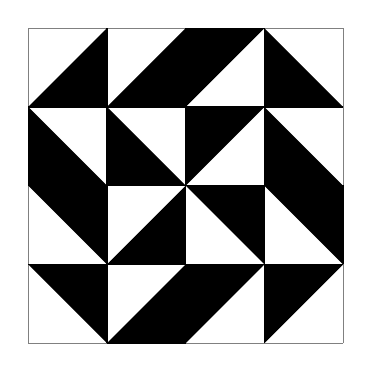
\begin{tikzpicture}[scale=1]
 \draw [step=1cm,gray,very thin](0,-1) grid (4,3); 
 \draw[opacity=1,fill=black](0,0)--(1,0)--(1,-1); 
 \draw[opacity=1,fill=black](0,1)--(1,1)--(1,0); 
 \draw[opacity=1,fill=black](1,1)--(0,1)--(0,2); 
 \draw[opacity=1,fill=black](1,3)--(1,2)--(0,2); 
 \draw[opacity=1,fill=black](2,0)--(2,-1)--(1,-1); 
 \draw[opacity=1,fill=black](2,1)--(2,0)--(1,0); 
 \draw[opacity=1,fill=black](2,1)--(1,1)--(1,2); 
 \draw[opacity=1,fill=black](2,3)--(2,2)--(1,2); 
 \draw[opacity=1,fill=black](2,-1)--(2,0)--(3,0); 
 \draw[opacity=1,fill=black](2,1)--(3,1)--(3,0); 
 \draw[opacity=1,fill=black](2,1)--(2,2)--(3,2); 
 \draw[opacity=1,fill=black](2,2)--(2,3)--(3,3); 
 \draw[opacity=1,fill=black](3,-1)--(3,0)--(4,0); 
 \draw[opacity=1,fill=black](3,1)--(4,1)--(4,0); 
 \draw[opacity=1,fill=black](4,1)--(3,1)--(3,2); 
 \draw[opacity=1,fill=black](4,2)--(3,2)--(3,3); 
\end{tikzpicture}

\textit{The 0011 pattern}
}
\end{center}

\chapter{Pattern families}

\noindent
We can group the 4x4 Truchet tile patterns with rotational symmetry into families where  tile patterns are considered to be in the same family if they would look the same without colour -- if each corresponding tile shares the same diagonal direction. The sequence that represents the family of a tile pattern can be found by taking the sequence of the tile pattern \textit{modulo} $2$. So, for example, the 16 tile patterns below are all members of the 0110 family. 

\vspace{1.2cm}

\marginnote{\centering\input{tiles/parent-0110.gtex}\\ \textit{The 0110 family pattern}}

{
\setlength{\tabcolsep}{3pt}
\renewcommand{\arraystretch}{2}
\input{example_family}
{\begin{center} \textit{The 0110 pattern family}\end{center}}
}

\newpage

%%
% Start the main matter (normal chapters)
%\mainmatter

%\input{tiles/0000.gtex}

\input{tiles/1000.gtex}

\section{0100}

\vspace{1cm}
\begin{center}
\begin{tabular}{cccc} 
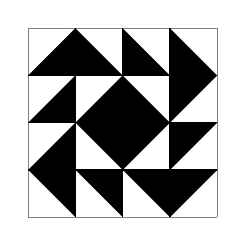
\begin{tikzpicture}[scale=0.6]
 \draw [step=1cm,gray,very thin](0,-1) grid (4,3); 
 \draw[opacity=1,fill=black](0,0)--(1,0)--(1,-1); 
 \draw[opacity=1,fill=black](1,1)--(1,0)--(0,0); 
 \draw[opacity=1,fill=black](1,2)--(1,1)--(0,1); 
 \draw[opacity=1,fill=black](1,3)--(1,2)--(0,2); 
 \draw[opacity=1,fill=black](1,0)--(2,0)--(2,-1); 
 \draw[opacity=1,fill=black](1,1)--(2,1)--(2,0); 
 \draw[opacity=1,fill=black](2,2)--(2,1)--(1,1); 
 \draw[opacity=1,fill=black](2,2)--(1,2)--(1,3); 
 \draw[opacity=1,fill=black](2,0)--(3,0)--(3,-1); 
 \draw[opacity=1,fill=black](2,0)--(2,1)--(3,1); 
 \draw[opacity=1,fill=black](3,1)--(2,1)--(2,2); 
 \draw[opacity=1,fill=black](3,2)--(2,2)--(2,3); 
 \draw[opacity=1,fill=black](3,-1)--(3,0)--(4,0); 
 \draw[opacity=1,fill=black](3,0)--(3,1)--(4,1); 
 \draw[opacity=1,fill=black](3,1)--(3,2)--(4,2); 
 \draw[opacity=1,fill=black](4,2)--(3,2)--(3,3); 
\end{tikzpicture} 
 & 
\begin{tikzpicture}[scale=0.6]
 \draw [step=1cm,gray,very thin](0,-1) grid (4,3); 
 \draw[opacity=1,fill=black](0,0)--(1,0)--(1,-1); 
 \draw[opacity=1,fill=black](1,1)--(1,0)--(0,0); 
 \draw[opacity=1,fill=black](1,2)--(1,1)--(0,1); 
 \draw[opacity=1,fill=black](1,3)--(1,2)--(0,2); 
 \draw[opacity=1,fill=black](1,0)--(2,0)--(2,-1); 
 \draw[opacity=1,fill=black](2,0)--(1,0)--(1,1); 
 \draw[opacity=1,fill=black](1,1)--(1,2)--(2,2); 
 \draw[opacity=1,fill=black](2,2)--(1,2)--(1,3); 
 \draw[opacity=1,fill=black](2,0)--(3,0)--(3,-1); 
 \draw[opacity=1,fill=black](3,1)--(3,0)--(2,0); 
 \draw[opacity=1,fill=black](2,2)--(3,2)--(3,1); 
 \draw[opacity=1,fill=black](3,2)--(2,2)--(2,3); 
 \draw[opacity=1,fill=black](3,-1)--(3,0)--(4,0); 
 \draw[opacity=1,fill=black](3,0)--(3,1)--(4,1); 
 \draw[opacity=1,fill=black](3,1)--(3,2)--(4,2); 
 \draw[opacity=1,fill=black](4,2)--(3,2)--(3,3); 
\end{tikzpicture} 
 & 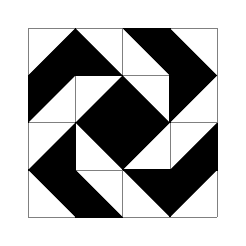
\begin{tikzpicture}[scale=0.6]
 \draw [step=1cm,gray,very thin](0,-1) grid (4,3); 
 \draw[opacity=1,fill=black](0,0)--(1,0)--(1,-1); 
 \draw[opacity=1,fill=black](1,1)--(1,0)--(0,0); 
 \draw[opacity=1,fill=black](0,1)--(0,2)--(1,2); 
 \draw[opacity=1,fill=black](1,3)--(1,2)--(0,2); 
 \draw[opacity=1,fill=black](2,-1)--(1,-1)--(1,0); 
 \draw[opacity=1,fill=black](1,1)--(2,1)--(2,0); 
 \draw[opacity=1,fill=black](2,2)--(2,1)--(1,1); 
 \draw[opacity=1,fill=black](2,2)--(1,2)--(1,3); 
 \draw[opacity=1,fill=black](2,0)--(3,0)--(3,-1); 
 \draw[opacity=1,fill=black](2,0)--(2,1)--(3,1); 
 \draw[opacity=1,fill=black](3,1)--(2,1)--(2,2); 
 \draw[opacity=1,fill=black](2,3)--(3,3)--(3,2); 
 \draw[opacity=1,fill=black](3,-1)--(3,0)--(4,0); 
 \draw[opacity=1,fill=black](4,1)--(4,0)--(3,0); 
 \draw[opacity=1,fill=black](3,1)--(3,2)--(4,2); 
 \draw[opacity=1,fill=black](4,2)--(3,2)--(3,3); 
\end{tikzpicture} 
 & 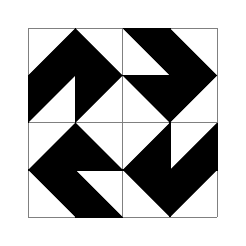
\begin{tikzpicture}[scale=0.6]
 \draw [step=1cm,gray,very thin](0,-1) grid (4,3); 
 \draw[opacity=1,fill=black](0,0)--(1,0)--(1,-1); 
 \draw[opacity=1,fill=black](1,1)--(1,0)--(0,0); 
 \draw[opacity=1,fill=black](0,1)--(0,2)--(1,2); 
 \draw[opacity=1,fill=black](1,3)--(1,2)--(0,2); 
 \draw[opacity=1,fill=black](2,-1)--(1,-1)--(1,0); 
 \draw[opacity=1,fill=black](2,0)--(1,0)--(1,1); 
 \draw[opacity=1,fill=black](1,1)--(1,2)--(2,2); 
 \draw[opacity=1,fill=black](2,2)--(1,2)--(1,3); 
 \draw[opacity=1,fill=black](2,0)--(3,0)--(3,-1); 
 \draw[opacity=1,fill=black](3,1)--(3,0)--(2,0); 
 \draw[opacity=1,fill=black](2,2)--(3,2)--(3,1); 
 \draw[opacity=1,fill=black](2,3)--(3,3)--(3,2); 
 \draw[opacity=1,fill=black](3,-1)--(3,0)--(4,0); 
 \draw[opacity=1,fill=black](4,1)--(4,0)--(3,0); 
 \draw[opacity=1,fill=black](3,1)--(3,2)--(4,2); 
 \draw[opacity=1,fill=black](4,2)--(3,2)--(3,3); 
\end{tikzpicture} 
\\ 
 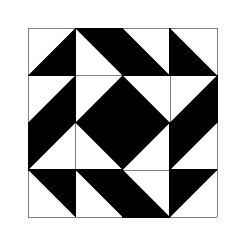
\begin{tikzpicture}[scale=0.6]
 \draw [step=1cm,gray,very thin](0,-1) grid (4,3); 
 \draw[opacity=1,fill=black](0,0)--(1,0)--(1,-1); 
 \draw[opacity=1,fill=black](0,0)--(0,1)--(1,1); 
 \draw[opacity=1,fill=black](1,2)--(1,1)--(0,1); 
 \draw[opacity=1,fill=black](1,3)--(1,2)--(0,2); 
 \draw[opacity=1,fill=black](1,0)--(2,0)--(2,-1); 
 \draw[opacity=1,fill=black](1,1)--(2,1)--(2,0); 
 \draw[opacity=1,fill=black](2,2)--(2,1)--(1,1); 
 \draw[opacity=1,fill=black](1,3)--(2,3)--(2,2); 
 \draw[opacity=1,fill=black](3,-1)--(2,-1)--(2,0); 
 \draw[opacity=1,fill=black](2,0)--(2,1)--(3,1); 
 \draw[opacity=1,fill=black](3,1)--(2,1)--(2,2); 
 \draw[opacity=1,fill=black](3,2)--(2,2)--(2,3); 
 \draw[opacity=1,fill=black](3,-1)--(3,0)--(4,0); 
 \draw[opacity=1,fill=black](3,0)--(3,1)--(4,1); 
 \draw[opacity=1,fill=black](4,2)--(4,1)--(3,1); 
 \draw[opacity=1,fill=black](4,2)--(3,2)--(3,3); 
\end{tikzpicture} 
 & 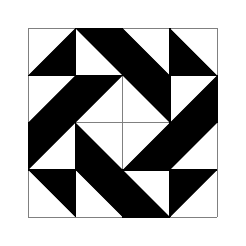
\begin{tikzpicture}[scale=0.6]
 \draw [step=1cm,gray,very thin](0,-1) grid (4,3); 
 \draw[opacity=1,fill=black](0,0)--(1,0)--(1,-1); 
 \draw[opacity=1,fill=black](0,0)--(0,1)--(1,1); 
 \draw[opacity=1,fill=black](1,2)--(1,1)--(0,1); 
 \draw[opacity=1,fill=black](1,3)--(1,2)--(0,2); 
 \draw[opacity=1,fill=black](1,0)--(2,0)--(2,-1); 
 \draw[opacity=1,fill=black](2,0)--(1,0)--(1,1); 
 \draw[opacity=1,fill=black](1,1)--(1,2)--(2,2); 
 \draw[opacity=1,fill=black](1,3)--(2,3)--(2,2); 
 \draw[opacity=1,fill=black](3,-1)--(2,-1)--(2,0); 
 \draw[opacity=1,fill=black](3,1)--(3,0)--(2,0); 
 \draw[opacity=1,fill=black](2,2)--(3,2)--(3,1); 
 \draw[opacity=1,fill=black](3,2)--(2,2)--(2,3); 
 \draw[opacity=1,fill=black](3,-1)--(3,0)--(4,0); 
 \draw[opacity=1,fill=black](3,0)--(3,1)--(4,1); 
 \draw[opacity=1,fill=black](4,2)--(4,1)--(3,1); 
 \draw[opacity=1,fill=black](4,2)--(3,2)--(3,3); 
\end{tikzpicture} 
 & 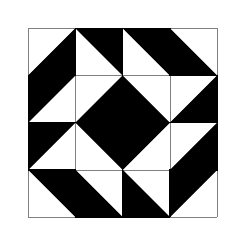
\begin{tikzpicture}[scale=0.6]
 \draw [step=1cm,gray,very thin](0,-1) grid (4,3); 
 \draw[opacity=1,fill=black](0,0)--(1,0)--(1,-1); 
 \draw[opacity=1,fill=black](0,0)--(0,1)--(1,1); 
 \draw[opacity=1,fill=black](0,1)--(0,2)--(1,2); 
 \draw[opacity=1,fill=black](1,3)--(1,2)--(0,2); 
 \draw[opacity=1,fill=black](2,-1)--(1,-1)--(1,0); 
 \draw[opacity=1,fill=black](1,1)--(2,1)--(2,0); 
 \draw[opacity=1,fill=black](2,2)--(2,1)--(1,1); 
 \draw[opacity=1,fill=black](1,3)--(2,3)--(2,2); 
 \draw[opacity=1,fill=black](3,-1)--(2,-1)--(2,0); 
 \draw[opacity=1,fill=black](2,0)--(2,1)--(3,1); 
 \draw[opacity=1,fill=black](3,1)--(2,1)--(2,2); 
 \draw[opacity=1,fill=black](2,3)--(3,3)--(3,2); 
 \draw[opacity=1,fill=black](3,-1)--(3,0)--(4,0); 
 \draw[opacity=1,fill=black](4,1)--(4,0)--(3,0); 
 \draw[opacity=1,fill=black](4,2)--(4,1)--(3,1); 
 \draw[opacity=1,fill=black](4,2)--(3,2)--(3,3); 
\end{tikzpicture} 
 & 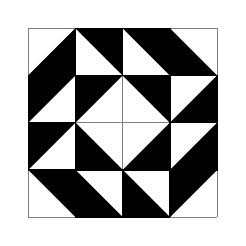
\begin{tikzpicture}[scale=0.6]
 \draw [step=1cm,gray,very thin](0,-1) grid (4,3); 
 \draw[opacity=1,fill=black](0,0)--(1,0)--(1,-1); 
 \draw[opacity=1,fill=black](0,0)--(0,1)--(1,1); 
 \draw[opacity=1,fill=black](0,1)--(0,2)--(1,2); 
 \draw[opacity=1,fill=black](1,3)--(1,2)--(0,2); 
 \draw[opacity=1,fill=black](2,-1)--(1,-1)--(1,0); 
 \draw[opacity=1,fill=black](2,0)--(1,0)--(1,1); 
 \draw[opacity=1,fill=black](1,1)--(1,2)--(2,2); 
 \draw[opacity=1,fill=black](1,3)--(2,3)--(2,2); 
 \draw[opacity=1,fill=black](3,-1)--(2,-1)--(2,0); 
 \draw[opacity=1,fill=black](3,1)--(3,0)--(2,0); 
 \draw[opacity=1,fill=black](2,2)--(3,2)--(3,1); 
 \draw[opacity=1,fill=black](2,3)--(3,3)--(3,2); 
 \draw[opacity=1,fill=black](3,-1)--(3,0)--(4,0); 
 \draw[opacity=1,fill=black](4,1)--(4,0)--(3,0); 
 \draw[opacity=1,fill=black](4,2)--(4,1)--(3,1); 
 \draw[opacity=1,fill=black](4,2)--(3,2)--(3,3); 
\end{tikzpicture} 
\\ 
 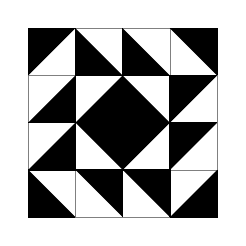
\begin{tikzpicture}[scale=0.6]
 \draw [step=1cm,gray,very thin](0,-1) grid (4,3); 
 \draw[opacity=1,fill=black](1,-1)--(0,-1)--(0,0); 
 \draw[opacity=1,fill=black](1,1)--(1,0)--(0,0); 
 \draw[opacity=1,fill=black](1,2)--(1,1)--(0,1); 
 \draw[opacity=1,fill=black](0,2)--(0,3)--(1,3); 
 \draw[opacity=1,fill=black](1,0)--(2,0)--(2,-1); 
 \draw[opacity=1,fill=black](1,1)--(2,1)--(2,0); 
 \draw[opacity=1,fill=black](2,2)--(2,1)--(1,1); 
 \draw[opacity=1,fill=black](2,2)--(1,2)--(1,3); 
 \draw[opacity=1,fill=black](2,0)--(3,0)--(3,-1); 
 \draw[opacity=1,fill=black](2,0)--(2,1)--(3,1); 
 \draw[opacity=1,fill=black](3,1)--(2,1)--(2,2); 
 \draw[opacity=1,fill=black](3,2)--(2,2)--(2,3); 
 \draw[opacity=1,fill=black](4,0)--(4,-1)--(3,-1); 
 \draw[opacity=1,fill=black](3,0)--(3,1)--(4,1); 
 \draw[opacity=1,fill=black](3,1)--(3,2)--(4,2); 
 \draw[opacity=1,fill=black](3,3)--(4,3)--(4,2); 
\end{tikzpicture} 
 & 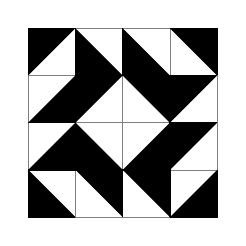
\begin{tikzpicture}[scale=0.6]
 \draw [step=1cm,gray,very thin](0,-1) grid (4,3); 
 \draw[opacity=1,fill=black](1,-1)--(0,-1)--(0,0); 
 \draw[opacity=1,fill=black](1,1)--(1,0)--(0,0); 
 \draw[opacity=1,fill=black](1,2)--(1,1)--(0,1); 
 \draw[opacity=1,fill=black](0,2)--(0,3)--(1,3); 
 \draw[opacity=1,fill=black](1,0)--(2,0)--(2,-1); 
 \draw[opacity=1,fill=black](2,0)--(1,0)--(1,1); 
 \draw[opacity=1,fill=black](1,1)--(1,2)--(2,2); 
 \draw[opacity=1,fill=black](2,2)--(1,2)--(1,3); 
 \draw[opacity=1,fill=black](2,0)--(3,0)--(3,-1); 
 \draw[opacity=1,fill=black](3,1)--(3,0)--(2,0); 
 \draw[opacity=1,fill=black](2,2)--(3,2)--(3,1); 
 \draw[opacity=1,fill=black](3,2)--(2,2)--(2,3); 
 \draw[opacity=1,fill=black](4,0)--(4,-1)--(3,-1); 
 \draw[opacity=1,fill=black](3,0)--(3,1)--(4,1); 
 \draw[opacity=1,fill=black](3,1)--(3,2)--(4,2); 
 \draw[opacity=1,fill=black](3,3)--(4,3)--(4,2); 
\end{tikzpicture} 
 & 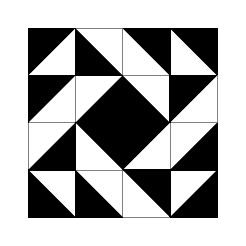
\begin{tikzpicture}[scale=0.6]
 \draw [step=1cm,gray,very thin](0,-1) grid (4,3); 
 \draw[opacity=1,fill=black](1,-1)--(0,-1)--(0,0); 
 \draw[opacity=1,fill=black](1,1)--(1,0)--(0,0); 
 \draw[opacity=1,fill=black](0,1)--(0,2)--(1,2); 
 \draw[opacity=1,fill=black](0,2)--(0,3)--(1,3); 
 \draw[opacity=1,fill=black](2,-1)--(1,-1)--(1,0); 
 \draw[opacity=1,fill=black](1,1)--(2,1)--(2,0); 
 \draw[opacity=1,fill=black](2,2)--(2,1)--(1,1); 
 \draw[opacity=1,fill=black](2,2)--(1,2)--(1,3); 
 \draw[opacity=1,fill=black](2,0)--(3,0)--(3,-1); 
 \draw[opacity=1,fill=black](2,0)--(2,1)--(3,1); 
 \draw[opacity=1,fill=black](3,1)--(2,1)--(2,2); 
 \draw[opacity=1,fill=black](2,3)--(3,3)--(3,2); 
 \draw[opacity=1,fill=black](4,0)--(4,-1)--(3,-1); 
 \draw[opacity=1,fill=black](4,1)--(4,0)--(3,0); 
 \draw[opacity=1,fill=black](3,1)--(3,2)--(4,2); 
 \draw[opacity=1,fill=black](3,3)--(4,3)--(4,2); 
\end{tikzpicture} 
 & 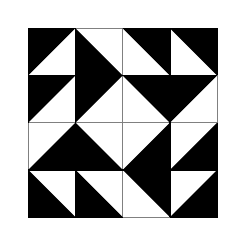
\begin{tikzpicture}[scale=0.6]
 \draw [step=1cm,gray,very thin](0,-1) grid (4,3); 
 \draw[opacity=1,fill=black](1,-1)--(0,-1)--(0,0); 
 \draw[opacity=1,fill=black](1,1)--(1,0)--(0,0); 
 \draw[opacity=1,fill=black](0,1)--(0,2)--(1,2); 
 \draw[opacity=1,fill=black](0,2)--(0,3)--(1,3); 
 \draw[opacity=1,fill=black](2,-1)--(1,-1)--(1,0); 
 \draw[opacity=1,fill=black](2,0)--(1,0)--(1,1); 
 \draw[opacity=1,fill=black](1,1)--(1,2)--(2,2); 
 \draw[opacity=1,fill=black](2,2)--(1,2)--(1,3); 
 \draw[opacity=1,fill=black](2,0)--(3,0)--(3,-1); 
 \draw[opacity=1,fill=black](3,1)--(3,0)--(2,0); 
 \draw[opacity=1,fill=black](2,2)--(3,2)--(3,1); 
 \draw[opacity=1,fill=black](2,3)--(3,3)--(3,2); 
 \draw[opacity=1,fill=black](4,0)--(4,-1)--(3,-1); 
 \draw[opacity=1,fill=black](4,1)--(4,0)--(3,0); 
 \draw[opacity=1,fill=black](3,1)--(3,2)--(4,2); 
 \draw[opacity=1,fill=black](3,3)--(4,3)--(4,2); 
\end{tikzpicture} 
\\ 
 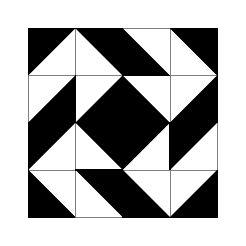
\begin{tikzpicture}[scale=0.6]
 \draw [step=1cm,gray,very thin](0,-1) grid (4,3); 
 \draw[opacity=1,fill=black](1,-1)--(0,-1)--(0,0); 
 \draw[opacity=1,fill=black](0,0)--(0,1)--(1,1); 
 \draw[opacity=1,fill=black](1,2)--(1,1)--(0,1); 
 \draw[opacity=1,fill=black](0,2)--(0,3)--(1,3); 
 \draw[opacity=1,fill=black](1,0)--(2,0)--(2,-1); 
 \draw[opacity=1,fill=black](1,1)--(2,1)--(2,0); 
 \draw[opacity=1,fill=black](2,2)--(2,1)--(1,1); 
 \draw[opacity=1,fill=black](1,3)--(2,3)--(2,2); 
 \draw[opacity=1,fill=black](3,-1)--(2,-1)--(2,0); 
 \draw[opacity=1,fill=black](2,0)--(2,1)--(3,1); 
 \draw[opacity=1,fill=black](3,1)--(2,1)--(2,2); 
 \draw[opacity=1,fill=black](3,2)--(2,2)--(2,3); 
 \draw[opacity=1,fill=black](4,0)--(4,-1)--(3,-1); 
 \draw[opacity=1,fill=black](3,0)--(3,1)--(4,1); 
 \draw[opacity=1,fill=black](4,2)--(4,1)--(3,1); 
 \draw[opacity=1,fill=black](3,3)--(4,3)--(4,2); 
\end{tikzpicture} 
 & 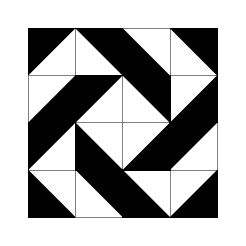
\begin{tikzpicture}[scale=0.6]
 \draw [step=1cm,gray,very thin](0,-1) grid (4,3); 
 \draw[opacity=1,fill=black](1,-1)--(0,-1)--(0,0); 
 \draw[opacity=1,fill=black](0,0)--(0,1)--(1,1); 
 \draw[opacity=1,fill=black](1,2)--(1,1)--(0,1); 
 \draw[opacity=1,fill=black](0,2)--(0,3)--(1,3); 
 \draw[opacity=1,fill=black](1,0)--(2,0)--(2,-1); 
 \draw[opacity=1,fill=black](2,0)--(1,0)--(1,1); 
 \draw[opacity=1,fill=black](1,1)--(1,2)--(2,2); 
 \draw[opacity=1,fill=black](1,3)--(2,3)--(2,2); 
 \draw[opacity=1,fill=black](3,-1)--(2,-1)--(2,0); 
 \draw[opacity=1,fill=black](3,1)--(3,0)--(2,0); 
 \draw[opacity=1,fill=black](2,2)--(3,2)--(3,1); 
 \draw[opacity=1,fill=black](3,2)--(2,2)--(2,3); 
 \draw[opacity=1,fill=black](4,0)--(4,-1)--(3,-1); 
 \draw[opacity=1,fill=black](3,0)--(3,1)--(4,1); 
 \draw[opacity=1,fill=black](4,2)--(4,1)--(3,1); 
 \draw[opacity=1,fill=black](3,3)--(4,3)--(4,2); 
\end{tikzpicture} 
 & 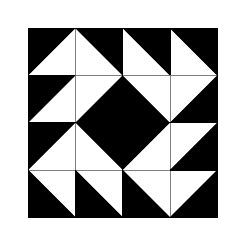
\begin{tikzpicture}[scale=0.6]
 \draw [step=1cm,gray,very thin](0,-1) grid (4,3); 
 \draw[opacity=1,fill=black](1,-1)--(0,-1)--(0,0); 
 \draw[opacity=1,fill=black](0,0)--(0,1)--(1,1); 
 \draw[opacity=1,fill=black](0,1)--(0,2)--(1,2); 
 \draw[opacity=1,fill=black](0,2)--(0,3)--(1,3); 
 \draw[opacity=1,fill=black](2,-1)--(1,-1)--(1,0); 
 \draw[opacity=1,fill=black](1,1)--(2,1)--(2,0); 
 \draw[opacity=1,fill=black](2,2)--(2,1)--(1,1); 
 \draw[opacity=1,fill=black](1,3)--(2,3)--(2,2); 
 \draw[opacity=1,fill=black](3,-1)--(2,-1)--(2,0); 
 \draw[opacity=1,fill=black](2,0)--(2,1)--(3,1); 
 \draw[opacity=1,fill=black](3,1)--(2,1)--(2,2); 
 \draw[opacity=1,fill=black](2,3)--(3,3)--(3,2); 
 \draw[opacity=1,fill=black](4,0)--(4,-1)--(3,-1); 
 \draw[opacity=1,fill=black](4,1)--(4,0)--(3,0); 
 \draw[opacity=1,fill=black](4,2)--(4,1)--(3,1); 
 \draw[opacity=1,fill=black](3,3)--(4,3)--(4,2); 
\end{tikzpicture} 
 & 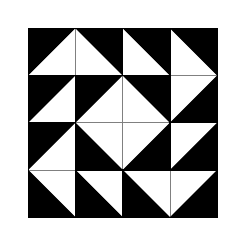
\begin{tikzpicture}[scale=0.6]
 \draw [step=1cm,gray,very thin](0,-1) grid (4,3); 
 \draw[opacity=1,fill=black](1,-1)--(0,-1)--(0,0); 
 \draw[opacity=1,fill=black](0,0)--(0,1)--(1,1); 
 \draw[opacity=1,fill=black](0,1)--(0,2)--(1,2); 
 \draw[opacity=1,fill=black](0,2)--(0,3)--(1,3); 
 \draw[opacity=1,fill=black](2,-1)--(1,-1)--(1,0); 
 \draw[opacity=1,fill=black](2,0)--(1,0)--(1,1); 
 \draw[opacity=1,fill=black](1,1)--(1,2)--(2,2); 
 \draw[opacity=1,fill=black](1,3)--(2,3)--(2,2); 
 \draw[opacity=1,fill=black](3,-1)--(2,-1)--(2,0); 
 \draw[opacity=1,fill=black](3,1)--(3,0)--(2,0); 
 \draw[opacity=1,fill=black](2,2)--(3,2)--(3,1); 
 \draw[opacity=1,fill=black](2,3)--(3,3)--(3,2); 
 \draw[opacity=1,fill=black](4,0)--(4,-1)--(3,-1); 
 \draw[opacity=1,fill=black](4,1)--(4,0)--(3,0); 
 \draw[opacity=1,fill=black](4,2)--(4,1)--(3,1); 
 \draw[opacity=1,fill=black](3,3)--(4,3)--(4,2); 
\end{tikzpicture} 
\\ 
 \end{tabular} 
\,\newline
\vspace{1cm}
{\Large
\begin{tabular}{cccc} 
0100 & 0102 & 0120 & 0122\\ 
 0300 & 0302 & 0320 & 0322\\ 
 2100 & 2102 & 2120 & 2122\\ 
 2300 & 2302 & 2320 & 2322\\ 
 \end{tabular} 
}
\,\newline
\vspace{1cm}
\begin{tabular}{cccc} 

\begin{tikzpicture}[scale=1]
 \draw[opacity=1,fill=black](0,-1)--(0,0)--(1,0); 
\end{tikzpicture} 
 & 
\begin{tikzpicture}[scale=1]
 \draw[opacity=1,fill=black](1,-1)--(0,-1)--(0,0); 
\end{tikzpicture} 
 & 
\begin{tikzpicture}[scale=1]
 \draw[opacity=1,fill=black](1,0)--(1,-1)--(0,-1); 
\end{tikzpicture} 
 & 
\begin{tikzpicture}[scale=1]
 \draw[opacity=1,fill=black](0,0)--(1,0)--(1,-1); 
\end{tikzpicture} 
\\ 
 \end{tabular} 
\end{center}

\newpage



\input{tiles/0010.gtex}

\input{tiles/0001.gtex}

\section{1100}

\begin{center}
\end{center}

\begin{tabular}{cccc} 
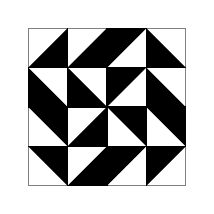
\begin{tikzpicture}[scale=0.5]
 \draw [step=1cm,gray,very thin](0,-1) grid (4,3); 
 \draw[opacity=1,fill=black](0,0)--(1,0)--(1,-1); 
 \draw[opacity=1,fill=black](0,1)--(1,1)--(1,0); 
 \draw[opacity=1,fill=black](1,1)--(0,1)--(0,2); 
 \draw[opacity=1,fill=black](1,3)--(1,2)--(0,2); 
 \draw[opacity=1,fill=black](2,0)--(2,-1)--(1,-1); 
 \draw[opacity=1,fill=black](2,1)--(2,0)--(1,0); 
 \draw[opacity=1,fill=black](2,1)--(1,1)--(1,2); 
 \draw[opacity=1,fill=black](2,3)--(2,2)--(1,2); 
 \draw[opacity=1,fill=black](2,-1)--(2,0)--(3,0); 
 \draw[opacity=1,fill=black](2,1)--(3,1)--(3,0); 
 \draw[opacity=1,fill=black](2,1)--(2,2)--(3,2); 
 \draw[opacity=1,fill=black](2,2)--(2,3)--(3,3); 
 \draw[opacity=1,fill=black](3,-1)--(3,0)--(4,0); 
 \draw[opacity=1,fill=black](3,1)--(4,1)--(4,0); 
 \draw[opacity=1,fill=black](4,1)--(3,1)--(3,2); 
 \draw[opacity=1,fill=black](4,2)--(3,2)--(3,3); 
\end{tikzpicture} 
 & 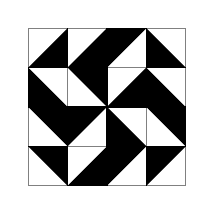
\begin{tikzpicture}[scale=0.5]
 \draw [step=1cm,gray,very thin](0,-1) grid (4,3); 
 \draw[opacity=1,fill=black](0,0)--(1,0)--(1,-1); 
 \draw[opacity=1,fill=black](0,1)--(1,1)--(1,0); 
 \draw[opacity=1,fill=black](1,1)--(0,1)--(0,2); 
 \draw[opacity=1,fill=black](1,3)--(1,2)--(0,2); 
 \draw[opacity=1,fill=black](2,0)--(2,-1)--(1,-1); 
 \draw[opacity=1,fill=black](1,0)--(1,1)--(2,1); 
 \draw[opacity=1,fill=black](1,2)--(2,2)--(2,1); 
 \draw[opacity=1,fill=black](2,3)--(2,2)--(1,2); 
 \draw[opacity=1,fill=black](2,-1)--(2,0)--(3,0); 
 \draw[opacity=1,fill=black](3,0)--(2,0)--(2,1); 
 \draw[opacity=1,fill=black](3,2)--(3,1)--(2,1); 
 \draw[opacity=1,fill=black](2,2)--(2,3)--(3,3); 
 \draw[opacity=1,fill=black](3,-1)--(3,0)--(4,0); 
 \draw[opacity=1,fill=black](3,1)--(4,1)--(4,0); 
 \draw[opacity=1,fill=black](4,1)--(3,1)--(3,2); 
 \draw[opacity=1,fill=black](4,2)--(3,2)--(3,3); 
\end{tikzpicture} 
 & 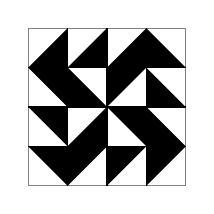
\begin{tikzpicture}[scale=0.5]
 \draw [step=1cm,gray,very thin](0,-1) grid (4,3); 
 \draw[opacity=1,fill=black](0,0)--(1,0)--(1,-1); 
 \draw[opacity=1,fill=black](0,1)--(1,1)--(1,0); 
 \draw[opacity=1,fill=black](0,2)--(1,2)--(1,1); 
 \draw[opacity=1,fill=black](1,3)--(1,2)--(0,2); 
 \draw[opacity=1,fill=black](1,-1)--(1,0)--(2,0); 
 \draw[opacity=1,fill=black](2,1)--(2,0)--(1,0); 
 \draw[opacity=1,fill=black](2,1)--(1,1)--(1,2); 
 \draw[opacity=1,fill=black](2,3)--(2,2)--(1,2); 
 \draw[opacity=1,fill=black](2,-1)--(2,0)--(3,0); 
 \draw[opacity=1,fill=black](2,1)--(3,1)--(3,0); 
 \draw[opacity=1,fill=black](2,1)--(2,2)--(3,2); 
 \draw[opacity=1,fill=black](3,3)--(3,2)--(2,2); 
 \draw[opacity=1,fill=black](3,-1)--(3,0)--(4,0); 
 \draw[opacity=1,fill=black](4,0)--(3,0)--(3,1); 
 \draw[opacity=1,fill=black](4,1)--(3,1)--(3,2); 
 \draw[opacity=1,fill=black](4,2)--(3,2)--(3,3); 
\end{tikzpicture} 
 & 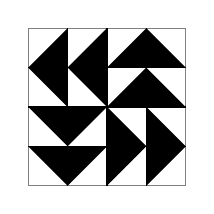
\begin{tikzpicture}[scale=0.5]
 \draw [step=1cm,gray,very thin](0,-1) grid (4,3); 
 \draw[opacity=1,fill=black](0,0)--(1,0)--(1,-1); 
 \draw[opacity=1,fill=black](0,1)--(1,1)--(1,0); 
 \draw[opacity=1,fill=black](0,2)--(1,2)--(1,1); 
 \draw[opacity=1,fill=black](1,3)--(1,2)--(0,2); 
 \draw[opacity=1,fill=black](1,-1)--(1,0)--(2,0); 
 \draw[opacity=1,fill=black](1,0)--(1,1)--(2,1); 
 \draw[opacity=1,fill=black](1,2)--(2,2)--(2,1); 
 \draw[opacity=1,fill=black](2,3)--(2,2)--(1,2); 
 \draw[opacity=1,fill=black](2,-1)--(2,0)--(3,0); 
 \draw[opacity=1,fill=black](3,0)--(2,0)--(2,1); 
 \draw[opacity=1,fill=black](3,2)--(3,1)--(2,1); 
 \draw[opacity=1,fill=black](3,3)--(3,2)--(2,2); 
 \draw[opacity=1,fill=black](3,-1)--(3,0)--(4,0); 
 \draw[opacity=1,fill=black](4,0)--(3,0)--(3,1); 
 \draw[opacity=1,fill=black](4,1)--(3,1)--(3,2); 
 \draw[opacity=1,fill=black](4,2)--(3,2)--(3,3); 
\end{tikzpicture} 
\\ 
 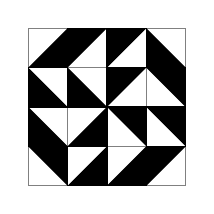
\begin{tikzpicture}[scale=0.5]
 \draw [step=1cm,gray,very thin](0,-1) grid (4,3); 
 \draw[opacity=1,fill=black](0,0)--(1,0)--(1,-1); 
 \draw[opacity=1,fill=black](1,0)--(0,0)--(0,1); 
 \draw[opacity=1,fill=black](1,1)--(0,1)--(0,2); 
 \draw[opacity=1,fill=black](1,3)--(1,2)--(0,2); 
 \draw[opacity=1,fill=black](2,0)--(2,-1)--(1,-1); 
 \draw[opacity=1,fill=black](2,1)--(2,0)--(1,0); 
 \draw[opacity=1,fill=black](2,1)--(1,1)--(1,2); 
 \draw[opacity=1,fill=black](1,2)--(1,3)--(2,3); 
 \draw[opacity=1,fill=black](3,0)--(3,-1)--(2,-1); 
 \draw[opacity=1,fill=black](2,1)--(3,1)--(3,0); 
 \draw[opacity=1,fill=black](2,1)--(2,2)--(3,2); 
 \draw[opacity=1,fill=black](2,2)--(2,3)--(3,3); 
 \draw[opacity=1,fill=black](3,-1)--(3,0)--(4,0); 
 \draw[opacity=1,fill=black](3,1)--(4,1)--(4,0); 
 \draw[opacity=1,fill=black](3,2)--(4,2)--(4,1); 
 \draw[opacity=1,fill=black](4,2)--(3,2)--(3,3); 
\end{tikzpicture} 
 & 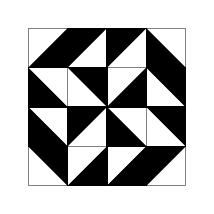
\begin{tikzpicture}[scale=0.5]
 \draw [step=1cm,gray,very thin](0,-1) grid (4,3); 
 \draw[opacity=1,fill=black](0,0)--(1,0)--(1,-1); 
 \draw[opacity=1,fill=black](1,0)--(0,0)--(0,1); 
 \draw[opacity=1,fill=black](1,1)--(0,1)--(0,2); 
 \draw[opacity=1,fill=black](1,3)--(1,2)--(0,2); 
 \draw[opacity=1,fill=black](2,0)--(2,-1)--(1,-1); 
 \draw[opacity=1,fill=black](1,0)--(1,1)--(2,1); 
 \draw[opacity=1,fill=black](1,2)--(2,2)--(2,1); 
 \draw[opacity=1,fill=black](1,2)--(1,3)--(2,3); 
 \draw[opacity=1,fill=black](3,0)--(3,-1)--(2,-1); 
 \draw[opacity=1,fill=black](3,0)--(2,0)--(2,1); 
 \draw[opacity=1,fill=black](3,2)--(3,1)--(2,1); 
 \draw[opacity=1,fill=black](2,2)--(2,3)--(3,3); 
 \draw[opacity=1,fill=black](3,-1)--(3,0)--(4,0); 
 \draw[opacity=1,fill=black](3,1)--(4,1)--(4,0); 
 \draw[opacity=1,fill=black](3,2)--(4,2)--(4,1); 
 \draw[opacity=1,fill=black](4,2)--(3,2)--(3,3); 
\end{tikzpicture} 
 & 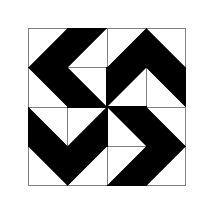
\begin{tikzpicture}[scale=0.5]
 \draw [step=1cm,gray,very thin](0,-1) grid (4,3); 
 \draw[opacity=1,fill=black](0,0)--(1,0)--(1,-1); 
 \draw[opacity=1,fill=black](1,0)--(0,0)--(0,1); 
 \draw[opacity=1,fill=black](0,2)--(1,2)--(1,1); 
 \draw[opacity=1,fill=black](1,3)--(1,2)--(0,2); 
 \draw[opacity=1,fill=black](1,-1)--(1,0)--(2,0); 
 \draw[opacity=1,fill=black](2,1)--(2,0)--(1,0); 
 \draw[opacity=1,fill=black](2,1)--(1,1)--(1,2); 
 \draw[opacity=1,fill=black](1,2)--(1,3)--(2,3); 
 \draw[opacity=1,fill=black](3,0)--(3,-1)--(2,-1); 
 \draw[opacity=1,fill=black](2,1)--(3,1)--(3,0); 
 \draw[opacity=1,fill=black](2,1)--(2,2)--(3,2); 
 \draw[opacity=1,fill=black](3,3)--(3,2)--(2,2); 
 \draw[opacity=1,fill=black](3,-1)--(3,0)--(4,0); 
 \draw[opacity=1,fill=black](4,0)--(3,0)--(3,1); 
 \draw[opacity=1,fill=black](3,2)--(4,2)--(4,1); 
 \draw[opacity=1,fill=black](4,2)--(3,2)--(3,3); 
\end{tikzpicture} 
 & 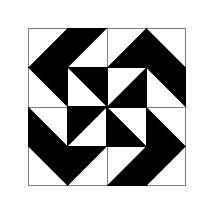
\begin{tikzpicture}[scale=0.5]
 \draw [step=1cm,gray,very thin](0,-1) grid (4,3); 
 \draw[opacity=1,fill=black](0,0)--(1,0)--(1,-1); 
 \draw[opacity=1,fill=black](1,0)--(0,0)--(0,1); 
 \draw[opacity=1,fill=black](0,2)--(1,2)--(1,1); 
 \draw[opacity=1,fill=black](1,3)--(1,2)--(0,2); 
 \draw[opacity=1,fill=black](1,-1)--(1,0)--(2,0); 
 \draw[opacity=1,fill=black](1,0)--(1,1)--(2,1); 
 \draw[opacity=1,fill=black](1,2)--(2,2)--(2,1); 
 \draw[opacity=1,fill=black](1,2)--(1,3)--(2,3); 
 \draw[opacity=1,fill=black](3,0)--(3,-1)--(2,-1); 
 \draw[opacity=1,fill=black](3,0)--(2,0)--(2,1); 
 \draw[opacity=1,fill=black](3,2)--(3,1)--(2,1); 
 \draw[opacity=1,fill=black](3,3)--(3,2)--(2,2); 
 \draw[opacity=1,fill=black](3,-1)--(3,0)--(4,0); 
 \draw[opacity=1,fill=black](4,0)--(3,0)--(3,1); 
 \draw[opacity=1,fill=black](3,2)--(4,2)--(4,1); 
 \draw[opacity=1,fill=black](4,2)--(3,2)--(3,3); 
\end{tikzpicture} 
\\ 
 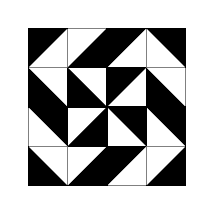
\begin{tikzpicture}[scale=0.5]
 \draw [step=1cm,gray,very thin](0,-1) grid (4,3); 
 \draw[opacity=1,fill=black](1,-1)--(0,-1)--(0,0); 
 \draw[opacity=1,fill=black](0,1)--(1,1)--(1,0); 
 \draw[opacity=1,fill=black](1,1)--(0,1)--(0,2); 
 \draw[opacity=1,fill=black](0,2)--(0,3)--(1,3); 
 \draw[opacity=1,fill=black](2,0)--(2,-1)--(1,-1); 
 \draw[opacity=1,fill=black](2,1)--(2,0)--(1,0); 
 \draw[opacity=1,fill=black](2,1)--(1,1)--(1,2); 
 \draw[opacity=1,fill=black](2,3)--(2,2)--(1,2); 
 \draw[opacity=1,fill=black](2,-1)--(2,0)--(3,0); 
 \draw[opacity=1,fill=black](2,1)--(3,1)--(3,0); 
 \draw[opacity=1,fill=black](2,1)--(2,2)--(3,2); 
 \draw[opacity=1,fill=black](2,2)--(2,3)--(3,3); 
 \draw[opacity=1,fill=black](4,0)--(4,-1)--(3,-1); 
 \draw[opacity=1,fill=black](3,1)--(4,1)--(4,0); 
 \draw[opacity=1,fill=black](4,1)--(3,1)--(3,2); 
 \draw[opacity=1,fill=black](3,3)--(4,3)--(4,2); 
\end{tikzpicture} 
 & 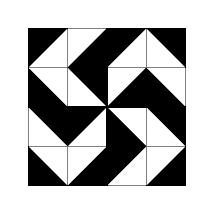
\begin{tikzpicture}[scale=0.5]
 \draw [step=1cm,gray,very thin](0,-1) grid (4,3); 
 \draw[opacity=1,fill=black](1,-1)--(0,-1)--(0,0); 
 \draw[opacity=1,fill=black](0,1)--(1,1)--(1,0); 
 \draw[opacity=1,fill=black](1,1)--(0,1)--(0,2); 
 \draw[opacity=1,fill=black](0,2)--(0,3)--(1,3); 
 \draw[opacity=1,fill=black](2,0)--(2,-1)--(1,-1); 
 \draw[opacity=1,fill=black](1,0)--(1,1)--(2,1); 
 \draw[opacity=1,fill=black](1,2)--(2,2)--(2,1); 
 \draw[opacity=1,fill=black](2,3)--(2,2)--(1,2); 
 \draw[opacity=1,fill=black](2,-1)--(2,0)--(3,0); 
 \draw[opacity=1,fill=black](3,0)--(2,0)--(2,1); 
 \draw[opacity=1,fill=black](3,2)--(3,1)--(2,1); 
 \draw[opacity=1,fill=black](2,2)--(2,3)--(3,3); 
 \draw[opacity=1,fill=black](4,0)--(4,-1)--(3,-1); 
 \draw[opacity=1,fill=black](3,1)--(4,1)--(4,0); 
 \draw[opacity=1,fill=black](4,1)--(3,1)--(3,2); 
 \draw[opacity=1,fill=black](3,3)--(4,3)--(4,2); 
\end{tikzpicture} 
 & 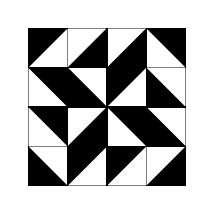
\begin{tikzpicture}[scale=0.5]
 \draw [step=1cm,gray,very thin](0,-1) grid (4,3); 
 \draw[opacity=1,fill=black](1,-1)--(0,-1)--(0,0); 
 \draw[opacity=1,fill=black](0,1)--(1,1)--(1,0); 
 \draw[opacity=1,fill=black](0,2)--(1,2)--(1,1); 
 \draw[opacity=1,fill=black](0,2)--(0,3)--(1,3); 
 \draw[opacity=1,fill=black](1,-1)--(1,0)--(2,0); 
 \draw[opacity=1,fill=black](2,1)--(2,0)--(1,0); 
 \draw[opacity=1,fill=black](2,1)--(1,1)--(1,2); 
 \draw[opacity=1,fill=black](2,3)--(2,2)--(1,2); 
 \draw[opacity=1,fill=black](2,-1)--(2,0)--(3,0); 
 \draw[opacity=1,fill=black](2,1)--(3,1)--(3,0); 
 \draw[opacity=1,fill=black](2,1)--(2,2)--(3,2); 
 \draw[opacity=1,fill=black](3,3)--(3,2)--(2,2); 
 \draw[opacity=1,fill=black](4,0)--(4,-1)--(3,-1); 
 \draw[opacity=1,fill=black](4,0)--(3,0)--(3,1); 
 \draw[opacity=1,fill=black](4,1)--(3,1)--(3,2); 
 \draw[opacity=1,fill=black](3,3)--(4,3)--(4,2); 
\end{tikzpicture} 
 & 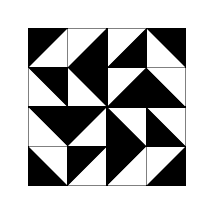
\begin{tikzpicture}[scale=0.5]
 \draw [step=1cm,gray,very thin](0,-1) grid (4,3); 
 \draw[opacity=1,fill=black](1,-1)--(0,-1)--(0,0); 
 \draw[opacity=1,fill=black](0,1)--(1,1)--(1,0); 
 \draw[opacity=1,fill=black](0,2)--(1,2)--(1,1); 
 \draw[opacity=1,fill=black](0,2)--(0,3)--(1,3); 
 \draw[opacity=1,fill=black](1,-1)--(1,0)--(2,0); 
 \draw[opacity=1,fill=black](1,0)--(1,1)--(2,1); 
 \draw[opacity=1,fill=black](1,2)--(2,2)--(2,1); 
 \draw[opacity=1,fill=black](2,3)--(2,2)--(1,2); 
 \draw[opacity=1,fill=black](2,-1)--(2,0)--(3,0); 
 \draw[opacity=1,fill=black](3,0)--(2,0)--(2,1); 
 \draw[opacity=1,fill=black](3,2)--(3,1)--(2,1); 
 \draw[opacity=1,fill=black](3,3)--(3,2)--(2,2); 
 \draw[opacity=1,fill=black](4,0)--(4,-1)--(3,-1); 
 \draw[opacity=1,fill=black](4,0)--(3,0)--(3,1); 
 \draw[opacity=1,fill=black](4,1)--(3,1)--(3,2); 
 \draw[opacity=1,fill=black](3,3)--(4,3)--(4,2); 
\end{tikzpicture} 
\\ 
 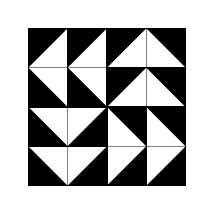
\begin{tikzpicture}[scale=0.5]
 \draw [step=1cm,gray,very thin](0,-1) grid (4,3); 
 \draw[opacity=1,fill=black](1,-1)--(0,-1)--(0,0); 
 \draw[opacity=1,fill=black](1,0)--(0,0)--(0,1); 
 \draw[opacity=1,fill=black](1,1)--(0,1)--(0,2); 
 \draw[opacity=1,fill=black](0,2)--(0,3)--(1,3); 
 \draw[opacity=1,fill=black](2,0)--(2,-1)--(1,-1); 
 \draw[opacity=1,fill=black](2,1)--(2,0)--(1,0); 
 \draw[opacity=1,fill=black](2,1)--(1,1)--(1,2); 
 \draw[opacity=1,fill=black](1,2)--(1,3)--(2,3); 
 \draw[opacity=1,fill=black](3,0)--(3,-1)--(2,-1); 
 \draw[opacity=1,fill=black](2,1)--(3,1)--(3,0); 
 \draw[opacity=1,fill=black](2,1)--(2,2)--(3,2); 
 \draw[opacity=1,fill=black](2,2)--(2,3)--(3,3); 
 \draw[opacity=1,fill=black](4,0)--(4,-1)--(3,-1); 
 \draw[opacity=1,fill=black](3,1)--(4,1)--(4,0); 
 \draw[opacity=1,fill=black](3,2)--(4,2)--(4,1); 
 \draw[opacity=1,fill=black](3,3)--(4,3)--(4,2); 
\end{tikzpicture} 
 & 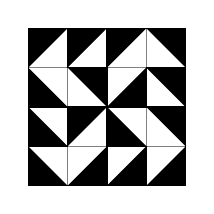
\begin{tikzpicture}[scale=0.5]
 \draw [step=1cm,gray,very thin](0,-1) grid (4,3); 
 \draw[opacity=1,fill=black](1,-1)--(0,-1)--(0,0); 
 \draw[opacity=1,fill=black](1,0)--(0,0)--(0,1); 
 \draw[opacity=1,fill=black](1,1)--(0,1)--(0,2); 
 \draw[opacity=1,fill=black](0,2)--(0,3)--(1,3); 
 \draw[opacity=1,fill=black](2,0)--(2,-1)--(1,-1); 
 \draw[opacity=1,fill=black](1,0)--(1,1)--(2,1); 
 \draw[opacity=1,fill=black](1,2)--(2,2)--(2,1); 
 \draw[opacity=1,fill=black](1,2)--(1,3)--(2,3); 
 \draw[opacity=1,fill=black](3,0)--(3,-1)--(2,-1); 
 \draw[opacity=1,fill=black](3,0)--(2,0)--(2,1); 
 \draw[opacity=1,fill=black](3,2)--(3,1)--(2,1); 
 \draw[opacity=1,fill=black](2,2)--(2,3)--(3,3); 
 \draw[opacity=1,fill=black](4,0)--(4,-1)--(3,-1); 
 \draw[opacity=1,fill=black](3,1)--(4,1)--(4,0); 
 \draw[opacity=1,fill=black](3,2)--(4,2)--(4,1); 
 \draw[opacity=1,fill=black](3,3)--(4,3)--(4,2); 
\end{tikzpicture} 
 & 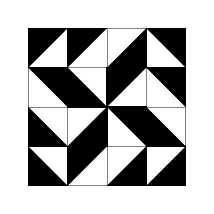
\begin{tikzpicture}[scale=0.5]
 \draw [step=1cm,gray,very thin](0,-1) grid (4,3); 
 \draw[opacity=1,fill=black](1,-1)--(0,-1)--(0,0); 
 \draw[opacity=1,fill=black](1,0)--(0,0)--(0,1); 
 \draw[opacity=1,fill=black](0,2)--(1,2)--(1,1); 
 \draw[opacity=1,fill=black](0,2)--(0,3)--(1,3); 
 \draw[opacity=1,fill=black](1,-1)--(1,0)--(2,0); 
 \draw[opacity=1,fill=black](2,1)--(2,0)--(1,0); 
 \draw[opacity=1,fill=black](2,1)--(1,1)--(1,2); 
 \draw[opacity=1,fill=black](1,2)--(1,3)--(2,3); 
 \draw[opacity=1,fill=black](3,0)--(3,-1)--(2,-1); 
 \draw[opacity=1,fill=black](2,1)--(3,1)--(3,0); 
 \draw[opacity=1,fill=black](2,1)--(2,2)--(3,2); 
 \draw[opacity=1,fill=black](3,3)--(3,2)--(2,2); 
 \draw[opacity=1,fill=black](4,0)--(4,-1)--(3,-1); 
 \draw[opacity=1,fill=black](4,0)--(3,0)--(3,1); 
 \draw[opacity=1,fill=black](3,2)--(4,2)--(4,1); 
 \draw[opacity=1,fill=black](3,3)--(4,3)--(4,2); 
\end{tikzpicture} 
 & 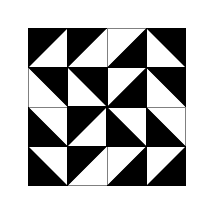
\begin{tikzpicture}[scale=0.5]
 \draw [step=1cm,gray,very thin](0,-1) grid (4,3); 
 \draw[opacity=1,fill=black](1,-1)--(0,-1)--(0,0); 
 \draw[opacity=1,fill=black](1,0)--(0,0)--(0,1); 
 \draw[opacity=1,fill=black](0,2)--(1,2)--(1,1); 
 \draw[opacity=1,fill=black](0,2)--(0,3)--(1,3); 
 \draw[opacity=1,fill=black](1,-1)--(1,0)--(2,0); 
 \draw[opacity=1,fill=black](1,0)--(1,1)--(2,1); 
 \draw[opacity=1,fill=black](1,2)--(2,2)--(2,1); 
 \draw[opacity=1,fill=black](1,2)--(1,3)--(2,3); 
 \draw[opacity=1,fill=black](3,0)--(3,-1)--(2,-1); 
 \draw[opacity=1,fill=black](3,0)--(2,0)--(2,1); 
 \draw[opacity=1,fill=black](3,2)--(3,1)--(2,1); 
 \draw[opacity=1,fill=black](3,3)--(3,2)--(2,2); 
 \draw[opacity=1,fill=black](4,0)--(4,-1)--(3,-1); 
 \draw[opacity=1,fill=black](4,0)--(3,0)--(3,1); 
 \draw[opacity=1,fill=black](3,2)--(4,2)--(4,1); 
 \draw[opacity=1,fill=black](3,3)--(4,3)--(4,2); 
\end{tikzpicture} 
\\ 
 \end{tabular} 

\begin{tabular}{cccc} 
0011 & 0013 & 0031 & 0033\\ 
 0211 & 0213 & 0231 & 0233\\ 
 2011 & 2013 & 2031 & 2033\\ 
 2211 & 2213 & 2231 & 2233\\ 
 \end{tabular} 

\newPage



\input{tiles/1010.gtex}

\section{1001}

\vspace{1cm}
\begin{center}
\begin{tabular}{cccc} 
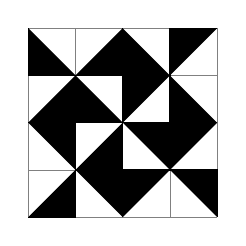
\begin{tikzpicture}[scale=0.6]
 \draw [step=1cm,gray,very thin](0,-1) grid (4,3); 
 \draw[opacity=1,fill=black](1,0)--(1,-1)--(0,-1); 
 \draw[opacity=1,fill=black](0,1)--(1,1)--(1,0); 
 \draw[opacity=1,fill=black](1,2)--(1,1)--(0,1); 
 \draw[opacity=1,fill=black](1,2)--(0,2)--(0,3); 
 \draw[opacity=1,fill=black](1,0)--(2,0)--(2,-1); 
 \draw[opacity=1,fill=black](2,1)--(2,0)--(1,0); 
 \draw[opacity=1,fill=black](2,1)--(1,1)--(1,2); 
 \draw[opacity=1,fill=black](2,3)--(2,2)--(1,2); 
 \draw[opacity=1,fill=black](2,-1)--(2,0)--(3,0); 
 \draw[opacity=1,fill=black](2,1)--(3,1)--(3,0); 
 \draw[opacity=1,fill=black](2,1)--(2,2)--(3,2); 
 \draw[opacity=1,fill=black](3,2)--(2,2)--(2,3); 
 \draw[opacity=1,fill=black](3,0)--(4,0)--(4,-1); 
 \draw[opacity=1,fill=black](3,0)--(3,1)--(4,1); 
 \draw[opacity=1,fill=black](4,1)--(3,1)--(3,2); 
 \draw[opacity=1,fill=black](3,2)--(3,3)--(4,3); 
\end{tikzpicture} 
 & 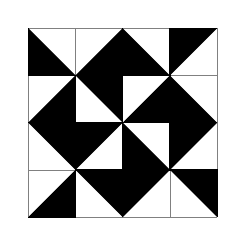
\begin{tikzpicture}[scale=0.6]
 \draw [step=1cm,gray,very thin](0,-1) grid (4,3); 
 \draw[opacity=1,fill=black](1,0)--(1,-1)--(0,-1); 
 \draw[opacity=1,fill=black](0,1)--(1,1)--(1,0); 
 \draw[opacity=1,fill=black](1,2)--(1,1)--(0,1); 
 \draw[opacity=1,fill=black](1,2)--(0,2)--(0,3); 
 \draw[opacity=1,fill=black](1,0)--(2,0)--(2,-1); 
 \draw[opacity=1,fill=black](1,0)--(1,1)--(2,1); 
 \draw[opacity=1,fill=black](1,2)--(2,2)--(2,1); 
 \draw[opacity=1,fill=black](2,3)--(2,2)--(1,2); 
 \draw[opacity=1,fill=black](2,-1)--(2,0)--(3,0); 
 \draw[opacity=1,fill=black](3,0)--(2,0)--(2,1); 
 \draw[opacity=1,fill=black](3,2)--(3,1)--(2,1); 
 \draw[opacity=1,fill=black](3,2)--(2,2)--(2,3); 
 \draw[opacity=1,fill=black](3,0)--(4,0)--(4,-1); 
 \draw[opacity=1,fill=black](3,0)--(3,1)--(4,1); 
 \draw[opacity=1,fill=black](4,1)--(3,1)--(3,2); 
 \draw[opacity=1,fill=black](3,2)--(3,3)--(4,3); 
\end{tikzpicture} 
 & 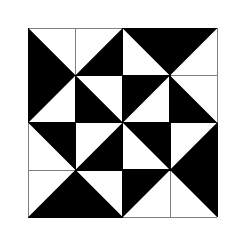
\begin{tikzpicture}[scale=0.6]
 \draw [step=1cm,gray,very thin](0,-1) grid (4,3); 
 \draw[opacity=1,fill=black](1,0)--(1,-1)--(0,-1); 
 \draw[opacity=1,fill=black](0,1)--(1,1)--(1,0); 
 \draw[opacity=1,fill=black](0,1)--(0,2)--(1,2); 
 \draw[opacity=1,fill=black](1,2)--(0,2)--(0,3); 
 \draw[opacity=1,fill=black](2,-1)--(1,-1)--(1,0); 
 \draw[opacity=1,fill=black](2,1)--(2,0)--(1,0); 
 \draw[opacity=1,fill=black](2,1)--(1,1)--(1,2); 
 \draw[opacity=1,fill=black](2,3)--(2,2)--(1,2); 
 \draw[opacity=1,fill=black](2,-1)--(2,0)--(3,0); 
 \draw[opacity=1,fill=black](2,1)--(3,1)--(3,0); 
 \draw[opacity=1,fill=black](2,1)--(2,2)--(3,2); 
 \draw[opacity=1,fill=black](2,3)--(3,3)--(3,2); 
 \draw[opacity=1,fill=black](3,0)--(4,0)--(4,-1); 
 \draw[opacity=1,fill=black](4,1)--(4,0)--(3,0); 
 \draw[opacity=1,fill=black](4,1)--(3,1)--(3,2); 
 \draw[opacity=1,fill=black](3,2)--(3,3)--(4,3); 
\end{tikzpicture} 
 & 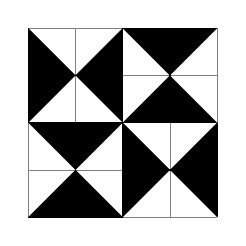
\begin{tikzpicture}[scale=0.6]
 \draw [step=1cm,gray,very thin](0,-1) grid (4,3); 
 \draw[opacity=1,fill=black](1,0)--(1,-1)--(0,-1); 
 \draw[opacity=1,fill=black](0,1)--(1,1)--(1,0); 
 \draw[opacity=1,fill=black](0,1)--(0,2)--(1,2); 
 \draw[opacity=1,fill=black](1,2)--(0,2)--(0,3); 
 \draw[opacity=1,fill=black](2,-1)--(1,-1)--(1,0); 
 \draw[opacity=1,fill=black](1,0)--(1,1)--(2,1); 
 \draw[opacity=1,fill=black](1,2)--(2,2)--(2,1); 
 \draw[opacity=1,fill=black](2,3)--(2,2)--(1,2); 
 \draw[opacity=1,fill=black](2,-1)--(2,0)--(3,0); 
 \draw[opacity=1,fill=black](3,0)--(2,0)--(2,1); 
 \draw[opacity=1,fill=black](3,2)--(3,1)--(2,1); 
 \draw[opacity=1,fill=black](2,3)--(3,3)--(3,2); 
 \draw[opacity=1,fill=black](3,0)--(4,0)--(4,-1); 
 \draw[opacity=1,fill=black](4,1)--(4,0)--(3,0); 
 \draw[opacity=1,fill=black](4,1)--(3,1)--(3,2); 
 \draw[opacity=1,fill=black](3,2)--(3,3)--(4,3); 
\end{tikzpicture} 
\\ 
 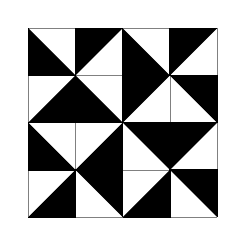
\begin{tikzpicture}[scale=0.6]
 \draw [step=1cm,gray,very thin](0,-1) grid (4,3); 
 \draw[opacity=1,fill=black](1,0)--(1,-1)--(0,-1); 
 \draw[opacity=1,fill=black](1,0)--(0,0)--(0,1); 
 \draw[opacity=1,fill=black](1,2)--(1,1)--(0,1); 
 \draw[opacity=1,fill=black](1,2)--(0,2)--(0,3); 
 \draw[opacity=1,fill=black](1,0)--(2,0)--(2,-1); 
 \draw[opacity=1,fill=black](2,1)--(2,0)--(1,0); 
 \draw[opacity=1,fill=black](2,1)--(1,1)--(1,2); 
 \draw[opacity=1,fill=black](1,2)--(1,3)--(2,3); 
 \draw[opacity=1,fill=black](3,0)--(3,-1)--(2,-1); 
 \draw[opacity=1,fill=black](2,1)--(3,1)--(3,0); 
 \draw[opacity=1,fill=black](2,1)--(2,2)--(3,2); 
 \draw[opacity=1,fill=black](3,2)--(2,2)--(2,3); 
 \draw[opacity=1,fill=black](3,0)--(4,0)--(4,-1); 
 \draw[opacity=1,fill=black](3,0)--(3,1)--(4,1); 
 \draw[opacity=1,fill=black](3,2)--(4,2)--(4,1); 
 \draw[opacity=1,fill=black](3,2)--(3,3)--(4,3); 
\end{tikzpicture} 
 & 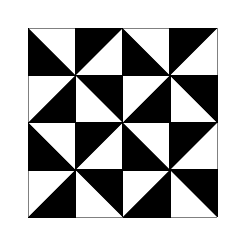
\begin{tikzpicture}[scale=0.6]
 \draw [step=1cm,gray,very thin](0,-1) grid (4,3); 
 \draw[opacity=1,fill=black](1,0)--(1,-1)--(0,-1); 
 \draw[opacity=1,fill=black](1,0)--(0,0)--(0,1); 
 \draw[opacity=1,fill=black](1,2)--(1,1)--(0,1); 
 \draw[opacity=1,fill=black](1,2)--(0,2)--(0,3); 
 \draw[opacity=1,fill=black](1,0)--(2,0)--(2,-1); 
 \draw[opacity=1,fill=black](1,0)--(1,1)--(2,1); 
 \draw[opacity=1,fill=black](1,2)--(2,2)--(2,1); 
 \draw[opacity=1,fill=black](1,2)--(1,3)--(2,3); 
 \draw[opacity=1,fill=black](3,0)--(3,-1)--(2,-1); 
 \draw[opacity=1,fill=black](3,0)--(2,0)--(2,1); 
 \draw[opacity=1,fill=black](3,2)--(3,1)--(2,1); 
 \draw[opacity=1,fill=black](3,2)--(2,2)--(2,3); 
 \draw[opacity=1,fill=black](3,0)--(4,0)--(4,-1); 
 \draw[opacity=1,fill=black](3,0)--(3,1)--(4,1); 
 \draw[opacity=1,fill=black](3,2)--(4,2)--(4,1); 
 \draw[opacity=1,fill=black](3,2)--(3,3)--(4,3); 
\end{tikzpicture} 
 & 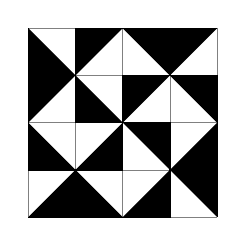
\begin{tikzpicture}[scale=0.6]
 \draw [step=1cm,gray,very thin](0,-1) grid (4,3); 
 \draw[opacity=1,fill=black](1,0)--(1,-1)--(0,-1); 
 \draw[opacity=1,fill=black](1,0)--(0,0)--(0,1); 
 \draw[opacity=1,fill=black](0,1)--(0,2)--(1,2); 
 \draw[opacity=1,fill=black](1,2)--(0,2)--(0,3); 
 \draw[opacity=1,fill=black](2,-1)--(1,-1)--(1,0); 
 \draw[opacity=1,fill=black](2,1)--(2,0)--(1,0); 
 \draw[opacity=1,fill=black](2,1)--(1,1)--(1,2); 
 \draw[opacity=1,fill=black](1,2)--(1,3)--(2,3); 
 \draw[opacity=1,fill=black](3,0)--(3,-1)--(2,-1); 
 \draw[opacity=1,fill=black](2,1)--(3,1)--(3,0); 
 \draw[opacity=1,fill=black](2,1)--(2,2)--(3,2); 
 \draw[opacity=1,fill=black](2,3)--(3,3)--(3,2); 
 \draw[opacity=1,fill=black](3,0)--(4,0)--(4,-1); 
 \draw[opacity=1,fill=black](4,1)--(4,0)--(3,0); 
 \draw[opacity=1,fill=black](3,2)--(4,2)--(4,1); 
 \draw[opacity=1,fill=black](3,2)--(3,3)--(4,3); 
\end{tikzpicture} 
 & 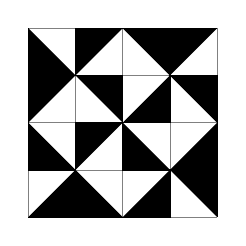
\begin{tikzpicture}[scale=0.6]
 \draw [step=1cm,gray,very thin](0,-1) grid (4,3); 
 \draw[opacity=1,fill=black](1,0)--(1,-1)--(0,-1); 
 \draw[opacity=1,fill=black](1,0)--(0,0)--(0,1); 
 \draw[opacity=1,fill=black](0,1)--(0,2)--(1,2); 
 \draw[opacity=1,fill=black](1,2)--(0,2)--(0,3); 
 \draw[opacity=1,fill=black](2,-1)--(1,-1)--(1,0); 
 \draw[opacity=1,fill=black](1,0)--(1,1)--(2,1); 
 \draw[opacity=1,fill=black](1,2)--(2,2)--(2,1); 
 \draw[opacity=1,fill=black](1,2)--(1,3)--(2,3); 
 \draw[opacity=1,fill=black](3,0)--(3,-1)--(2,-1); 
 \draw[opacity=1,fill=black](3,0)--(2,0)--(2,1); 
 \draw[opacity=1,fill=black](3,2)--(3,1)--(2,1); 
 \draw[opacity=1,fill=black](2,3)--(3,3)--(3,2); 
 \draw[opacity=1,fill=black](3,0)--(4,0)--(4,-1); 
 \draw[opacity=1,fill=black](4,1)--(4,0)--(3,0); 
 \draw[opacity=1,fill=black](3,2)--(4,2)--(4,1); 
 \draw[opacity=1,fill=black](3,2)--(3,3)--(4,3); 
\end{tikzpicture} 
\\ 
 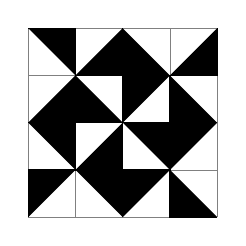
\begin{tikzpicture}[scale=0.6]
 \draw [step=1cm,gray,very thin](0,-1) grid (4,3); 
 \draw[opacity=1,fill=black](0,-1)--(0,0)--(1,0); 
 \draw[opacity=1,fill=black](0,1)--(1,1)--(1,0); 
 \draw[opacity=1,fill=black](1,2)--(1,1)--(0,1); 
 \draw[opacity=1,fill=black](0,3)--(1,3)--(1,2); 
 \draw[opacity=1,fill=black](1,0)--(2,0)--(2,-1); 
 \draw[opacity=1,fill=black](2,1)--(2,0)--(1,0); 
 \draw[opacity=1,fill=black](2,1)--(1,1)--(1,2); 
 \draw[opacity=1,fill=black](2,3)--(2,2)--(1,2); 
 \draw[opacity=1,fill=black](2,-1)--(2,0)--(3,0); 
 \draw[opacity=1,fill=black](2,1)--(3,1)--(3,0); 
 \draw[opacity=1,fill=black](2,1)--(2,2)--(3,2); 
 \draw[opacity=1,fill=black](3,2)--(2,2)--(2,3); 
 \draw[opacity=1,fill=black](4,-1)--(3,-1)--(3,0); 
 \draw[opacity=1,fill=black](3,0)--(3,1)--(4,1); 
 \draw[opacity=1,fill=black](4,1)--(3,1)--(3,2); 
 \draw[opacity=1,fill=black](4,3)--(4,2)--(3,2); 
\end{tikzpicture} 
 & 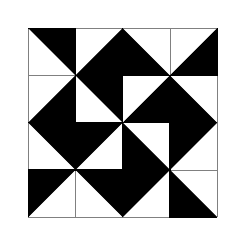
\begin{tikzpicture}[scale=0.6]
 \draw [step=1cm,gray,very thin](0,-1) grid (4,3); 
 \draw[opacity=1,fill=black](0,-1)--(0,0)--(1,0); 
 \draw[opacity=1,fill=black](0,1)--(1,1)--(1,0); 
 \draw[opacity=1,fill=black](1,2)--(1,1)--(0,1); 
 \draw[opacity=1,fill=black](0,3)--(1,3)--(1,2); 
 \draw[opacity=1,fill=black](1,0)--(2,0)--(2,-1); 
 \draw[opacity=1,fill=black](1,0)--(1,1)--(2,1); 
 \draw[opacity=1,fill=black](1,2)--(2,2)--(2,1); 
 \draw[opacity=1,fill=black](2,3)--(2,2)--(1,2); 
 \draw[opacity=1,fill=black](2,-1)--(2,0)--(3,0); 
 \draw[opacity=1,fill=black](3,0)--(2,0)--(2,1); 
 \draw[opacity=1,fill=black](3,2)--(3,1)--(2,1); 
 \draw[opacity=1,fill=black](3,2)--(2,2)--(2,3); 
 \draw[opacity=1,fill=black](4,-1)--(3,-1)--(3,0); 
 \draw[opacity=1,fill=black](3,0)--(3,1)--(4,1); 
 \draw[opacity=1,fill=black](4,1)--(3,1)--(3,2); 
 \draw[opacity=1,fill=black](4,3)--(4,2)--(3,2); 
\end{tikzpicture} 
 & 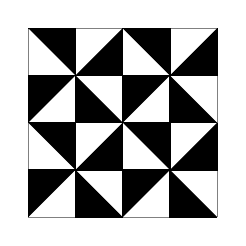
\begin{tikzpicture}[scale=0.6]
 \draw [step=1cm,gray,very thin](0,-1) grid (4,3); 
 \draw[opacity=1,fill=black](0,-1)--(0,0)--(1,0); 
 \draw[opacity=1,fill=black](0,1)--(1,1)--(1,0); 
 \draw[opacity=1,fill=black](0,1)--(0,2)--(1,2); 
 \draw[opacity=1,fill=black](0,3)--(1,3)--(1,2); 
 \draw[opacity=1,fill=black](2,-1)--(1,-1)--(1,0); 
 \draw[opacity=1,fill=black](2,1)--(2,0)--(1,0); 
 \draw[opacity=1,fill=black](2,1)--(1,1)--(1,2); 
 \draw[opacity=1,fill=black](2,3)--(2,2)--(1,2); 
 \draw[opacity=1,fill=black](2,-1)--(2,0)--(3,0); 
 \draw[opacity=1,fill=black](2,1)--(3,1)--(3,0); 
 \draw[opacity=1,fill=black](2,1)--(2,2)--(3,2); 
 \draw[opacity=1,fill=black](2,3)--(3,3)--(3,2); 
 \draw[opacity=1,fill=black](4,-1)--(3,-1)--(3,0); 
 \draw[opacity=1,fill=black](4,1)--(4,0)--(3,0); 
 \draw[opacity=1,fill=black](4,1)--(3,1)--(3,2); 
 \draw[opacity=1,fill=black](4,3)--(4,2)--(3,2); 
\end{tikzpicture} 
 & 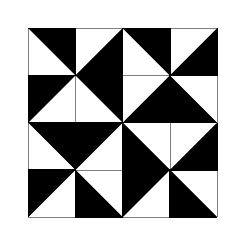
\begin{tikzpicture}[scale=0.6]
 \draw [step=1cm,gray,very thin](0,-1) grid (4,3); 
 \draw[opacity=1,fill=black](0,-1)--(0,0)--(1,0); 
 \draw[opacity=1,fill=black](0,1)--(1,1)--(1,0); 
 \draw[opacity=1,fill=black](0,1)--(0,2)--(1,2); 
 \draw[opacity=1,fill=black](0,3)--(1,3)--(1,2); 
 \draw[opacity=1,fill=black](2,-1)--(1,-1)--(1,0); 
 \draw[opacity=1,fill=black](1,0)--(1,1)--(2,1); 
 \draw[opacity=1,fill=black](1,2)--(2,2)--(2,1); 
 \draw[opacity=1,fill=black](2,3)--(2,2)--(1,2); 
 \draw[opacity=1,fill=black](2,-1)--(2,0)--(3,0); 
 \draw[opacity=1,fill=black](3,0)--(2,0)--(2,1); 
 \draw[opacity=1,fill=black](3,2)--(3,1)--(2,1); 
 \draw[opacity=1,fill=black](2,3)--(3,3)--(3,2); 
 \draw[opacity=1,fill=black](4,-1)--(3,-1)--(3,0); 
 \draw[opacity=1,fill=black](4,1)--(4,0)--(3,0); 
 \draw[opacity=1,fill=black](4,1)--(3,1)--(3,2); 
 \draw[opacity=1,fill=black](4,3)--(4,2)--(3,2); 
\end{tikzpicture} 
\\ 
 \begin{tikzpicture}[scale=0.6]
 \draw [step=1cm,gray,very thin](0,-1) grid (4,3); 
 \draw[opacity=1,fill=black](0,-1)--(0,0)--(1,0); 
 \draw[opacity=1,fill=black](1,0)--(0,0)--(0,1); 
 \draw[opacity=1,fill=black](1,2)--(1,1)--(0,1); 
 \draw[opacity=1,fill=black](0,3)--(1,3)--(1,2); 
 \draw[opacity=1,fill=black](1,0)--(2,0)--(2,-1); 
 \draw[opacity=1,fill=black](2,1)--(2,0)--(1,0); 
 \draw[opacity=1,fill=black](2,1)--(1,1)--(1,2); 
 \draw[opacity=1,fill=black](1,2)--(1,3)--(2,3); 
 \draw[opacity=1,fill=black](3,0)--(3,-1)--(2,-1); 
 \draw[opacity=1,fill=black](2,1)--(3,1)--(3,0); 
 \draw[opacity=1,fill=black](2,1)--(2,2)--(3,2); 
 \draw[opacity=1,fill=black](3,2)--(2,2)--(2,3); 
 \draw[opacity=1,fill=black](4,-1)--(3,-1)--(3,0); 
 \draw[opacity=1,fill=black](3,0)--(3,1)--(4,1); 
 \draw[opacity=1,fill=black](3,2)--(4,2)--(4,1); 
 \draw[opacity=1,fill=black](4,3)--(4,2)--(3,2); 
\end{tikzpicture} 
 & \begin{tikzpicture}[scale=0.6]
 \draw [step=1cm,gray,very thin](0,-1) grid (4,3); 
 \draw[opacity=1,fill=black](0,-1)--(0,0)--(1,0); 
 \draw[opacity=1,fill=black](1,0)--(0,0)--(0,1); 
 \draw[opacity=1,fill=black](1,2)--(1,1)--(0,1); 
 \draw[opacity=1,fill=black](0,3)--(1,3)--(1,2); 
 \draw[opacity=1,fill=black](1,0)--(2,0)--(2,-1); 
 \draw[opacity=1,fill=black](1,0)--(1,1)--(2,1); 
 \draw[opacity=1,fill=black](1,2)--(2,2)--(2,1); 
 \draw[opacity=1,fill=black](1,2)--(1,3)--(2,3); 
 \draw[opacity=1,fill=black](3,0)--(3,-1)--(2,-1); 
 \draw[opacity=1,fill=black](3,0)--(2,0)--(2,1); 
 \draw[opacity=1,fill=black](3,2)--(3,1)--(2,1); 
 \draw[opacity=1,fill=black](3,2)--(2,2)--(2,3); 
 \draw[opacity=1,fill=black](4,-1)--(3,-1)--(3,0); 
 \draw[opacity=1,fill=black](3,0)--(3,1)--(4,1); 
 \draw[opacity=1,fill=black](3,2)--(4,2)--(4,1); 
 \draw[opacity=1,fill=black](4,3)--(4,2)--(3,2); 
\end{tikzpicture} 
 & \begin{tikzpicture}[scale=0.6]
 \draw [step=1cm,gray,very thin](0,-1) grid (4,3); 
 \draw[opacity=1,fill=black](0,-1)--(0,0)--(1,0); 
 \draw[opacity=1,fill=black](1,0)--(0,0)--(0,1); 
 \draw[opacity=1,fill=black](0,1)--(0,2)--(1,2); 
 \draw[opacity=1,fill=black](0,3)--(1,3)--(1,2); 
 \draw[opacity=1,fill=black](2,-1)--(1,-1)--(1,0); 
 \draw[opacity=1,fill=black](2,1)--(2,0)--(1,0); 
 \draw[opacity=1,fill=black](2,1)--(1,1)--(1,2); 
 \draw[opacity=1,fill=black](1,2)--(1,3)--(2,3); 
 \draw[opacity=1,fill=black](3,0)--(3,-1)--(2,-1); 
 \draw[opacity=1,fill=black](2,1)--(3,1)--(3,0); 
 \draw[opacity=1,fill=black](2,1)--(2,2)--(3,2); 
 \draw[opacity=1,fill=black](2,3)--(3,3)--(3,2); 
 \draw[opacity=1,fill=black](4,-1)--(3,-1)--(3,0); 
 \draw[opacity=1,fill=black](4,1)--(4,0)--(3,0); 
 \draw[opacity=1,fill=black](3,2)--(4,2)--(4,1); 
 \draw[opacity=1,fill=black](4,3)--(4,2)--(3,2); 
\end{tikzpicture} 
 & \begin{tikzpicture}[scale=0.6]
 \draw [step=1cm,gray,very thin](0,-1) grid (4,3); 
 \draw[opacity=1,fill=black](0,-1)--(0,0)--(1,0); 
 \draw[opacity=1,fill=black](1,0)--(0,0)--(0,1); 
 \draw[opacity=1,fill=black](0,1)--(0,2)--(1,2); 
 \draw[opacity=1,fill=black](0,3)--(1,3)--(1,2); 
 \draw[opacity=1,fill=black](2,-1)--(1,-1)--(1,0); 
 \draw[opacity=1,fill=black](1,0)--(1,1)--(2,1); 
 \draw[opacity=1,fill=black](1,2)--(2,2)--(2,1); 
 \draw[opacity=1,fill=black](1,2)--(1,3)--(2,3); 
 \draw[opacity=1,fill=black](3,0)--(3,-1)--(2,-1); 
 \draw[opacity=1,fill=black](3,0)--(2,0)--(2,1); 
 \draw[opacity=1,fill=black](3,2)--(3,1)--(2,1); 
 \draw[opacity=1,fill=black](2,3)--(3,3)--(3,2); 
 \draw[opacity=1,fill=black](4,-1)--(3,-1)--(3,0); 
 \draw[opacity=1,fill=black](4,1)--(4,0)--(3,0); 
 \draw[opacity=1,fill=black](3,2)--(4,2)--(4,1); 
 \draw[opacity=1,fill=black](4,3)--(4,2)--(3,2); 
\end{tikzpicture} 
\\ 
 \end{tabular} 
\,\newline
\vspace{1cm}
{\Large
\begin{tabular}{cccc} 
1001 & 1003 & 1021 & 1023\\ 
 1201 & 1203 & 1221 & 1223\\ 
 3001 & 3003 & 3021 & 3023\\ 
 3201 & 3203 & 3221 & 3223\\ 
 \end{tabular} 
}
\,\newline
\vspace{1cm}
\begin{tabular}{cccc} 
\begin{tikzpicture}[scale=1]
 \draw[opacity=1,fill=black](0,-1)--(0,0)--(1,0); 
\end{tikzpicture} 
 & \begin{tikzpicture}[scale=1]
 \draw[opacity=1,fill=black](1,-1)--(0,-1)--(0,0); 
\end{tikzpicture} 
 & \begin{tikzpicture}[scale=1]
 \draw[opacity=1,fill=black](1,0)--(1,-1)--(0,-1); 
\end{tikzpicture} 
 & \begin{tikzpicture}[scale=1]
 \draw[opacity=1,fill=black](0,0)--(1,0)--(1,-1); 
\end{tikzpicture} 
\\ 
 \end{tabular} 
\end{center}

\newpage




% \newpage
% \,
% \vspace{2cm}
% \begin{center}
% \setlength{\tabcolsep}{2pt}
% \marginnote[0.8\baselineskip]{
% \begin{center}
% \input{tiles/parentTable.gtex}
% \end{center}
% }
% \input{tiles/bigTable.gtex}
% \end{center}
\chapter{Friezes of Truchet patterns}

\noindent
Each 4x4 Truchet pattern can be treated like a tile and used in a larger pattern. A \textit{frieze} is a horizontal strip of the same tile pattern repeated. Friezes of 4x4 Truchet pattern tiles with rotational symmetry can be quite striking, and have some interesting characteristics. 

\vspace{0.5cm}
\noindent
In frieze of more than one row of a primary tile reveals a secondary tile pattern that appears as another horizontal strip of 4x4 Truchet tile patterns nestled between the rows of primary tiles. Below, a frieze of 2223 tiles has a secondary pattern of 1000 tiles.
\,

\vspace{0.5cm}
\input{sample_frieze}

\vspace{0.5cm}
\noindent
Frieze patterns made from tiles of a particular family will have secondary tiles that also have rotational symmetry and that are from the same family. For example, frieze patters from the family 0001 will have secondary patterns from the family 1000. 
\marginnote{\centering\input{secondary_positions}} 

\vspace{0.5cm}
\noindent
You can compute the secondary frieze tile pattern of a given tile by reversing the digits of the tile label and adding 2 to each digit, modulo 4. This is because the label of the secondary frieze tile pattern comes from the top right corner of the primary tile pattern. 

\vspace{0.5cm}
\noindent
If tile \textit{t} is the primary tile in a frieze pattern and \textit{s} is the secondary, then \textit{t} will be the secondary tile in the frieze pattern formed by \textit{s}. This effectively reduces the total number of unique frieze patterns to 136, these patterns are shown on the pages that follow.
\newpage

%\input{ch2_generated_files/frieze_0000.gtex}

\input{ch2_generated_files/frieze_0001.gtex}

\input{ch2_generated_files/frieze_0010.gtex}

\input{ch2_generated_files/frieze_0011.gtex}

\input{ch2_generated_files/frieze_0101.gtex}

\input{ch2_generated_files/frieze_0110.gtex}

\input{ch2_generated_files/frieze_0111.gtex}

\input{ch2_generated_files/frieze_1001.gtex}

\input{ch2_generated_files/frieze_1011.gtex}

\input{ch2_generated_files/frieze_1111.gtex}



\chapter{Some designs}

{
\setlength{\tabcolsep}{0pt}
\renewcommand{\arraystretch}{0}
\section{Design using 2123 and 2130}

\marginnote[\baselineskip]{\centering\input{tiles/2123-alone.gtex}\\
2123}
\marginnote[\baselineskip]{\centering\input{tiles/2130-alone.gtex}\\
2130}
\begin{center}

\begin{center}

\input{tiles/2123-2130-design.gtex}
\end{center}

\end{center}

\vspace{0.2cm}



\backmatter
\nocite{*}
\bibliography{references}
\bibliographystyle{plainnat}
%\printindex

\end{document}
